\subsubsection{Benchmark \#\counter{feelppWP1benchcounter}: Elliptic linear PDE : Thermal bridges}
\label{sec:WP1:Feelpp:benchmark:thermal_bridges}
\paragraph{Description:} %Briefly describe the benchmark case, including the problem size, target architecture (e.g., CPU, GPU), and the input data. Mention the specific goals of the benchmark (e.g., testing scalability, energy efficiency).

The benchmark known as "thermal bridges" is an example of an application that
enables us to validate numerical simulation tools using \Feelpp. We have
developed tests based on the ISO 10211:2017 standard
\fullcite{noauthor_iso_2017}, which provides methodologies for evaluating
thermal bridges in building construction.

Thermal bridges are areas within a building envelope where heat
flow is different compared to adjacent areas, often resulting in increased heat
loss or unwanted condensation.
The standard is intended to ensure that thermal
bridges simulation are accurately computed. It provides reference values (and tolerance) on heat
temperature and heat flux at several location of the geometry.

At the mathematical level, this application requires finding the numerical
solution of an elliptic linear PDE (i.e. the heat equation). We employ a
finite element method based on continuous Lagrange Finite Element of order 1,2
and 3 (denoted by $P_1$,$P_2$,$P_3$). And we analyzed the execution time of the
main components of the simulation.

The \Cref{fig:wp1:feelpp:thermal_bridges:visualization} illustrate the geometry
used, the 3D temperature field solution, and an example of mesh partitioning.


\begin{figure}[h]
  \centering
  \begin{subfigure}[c]{0.49\textwidth}
    \centering
    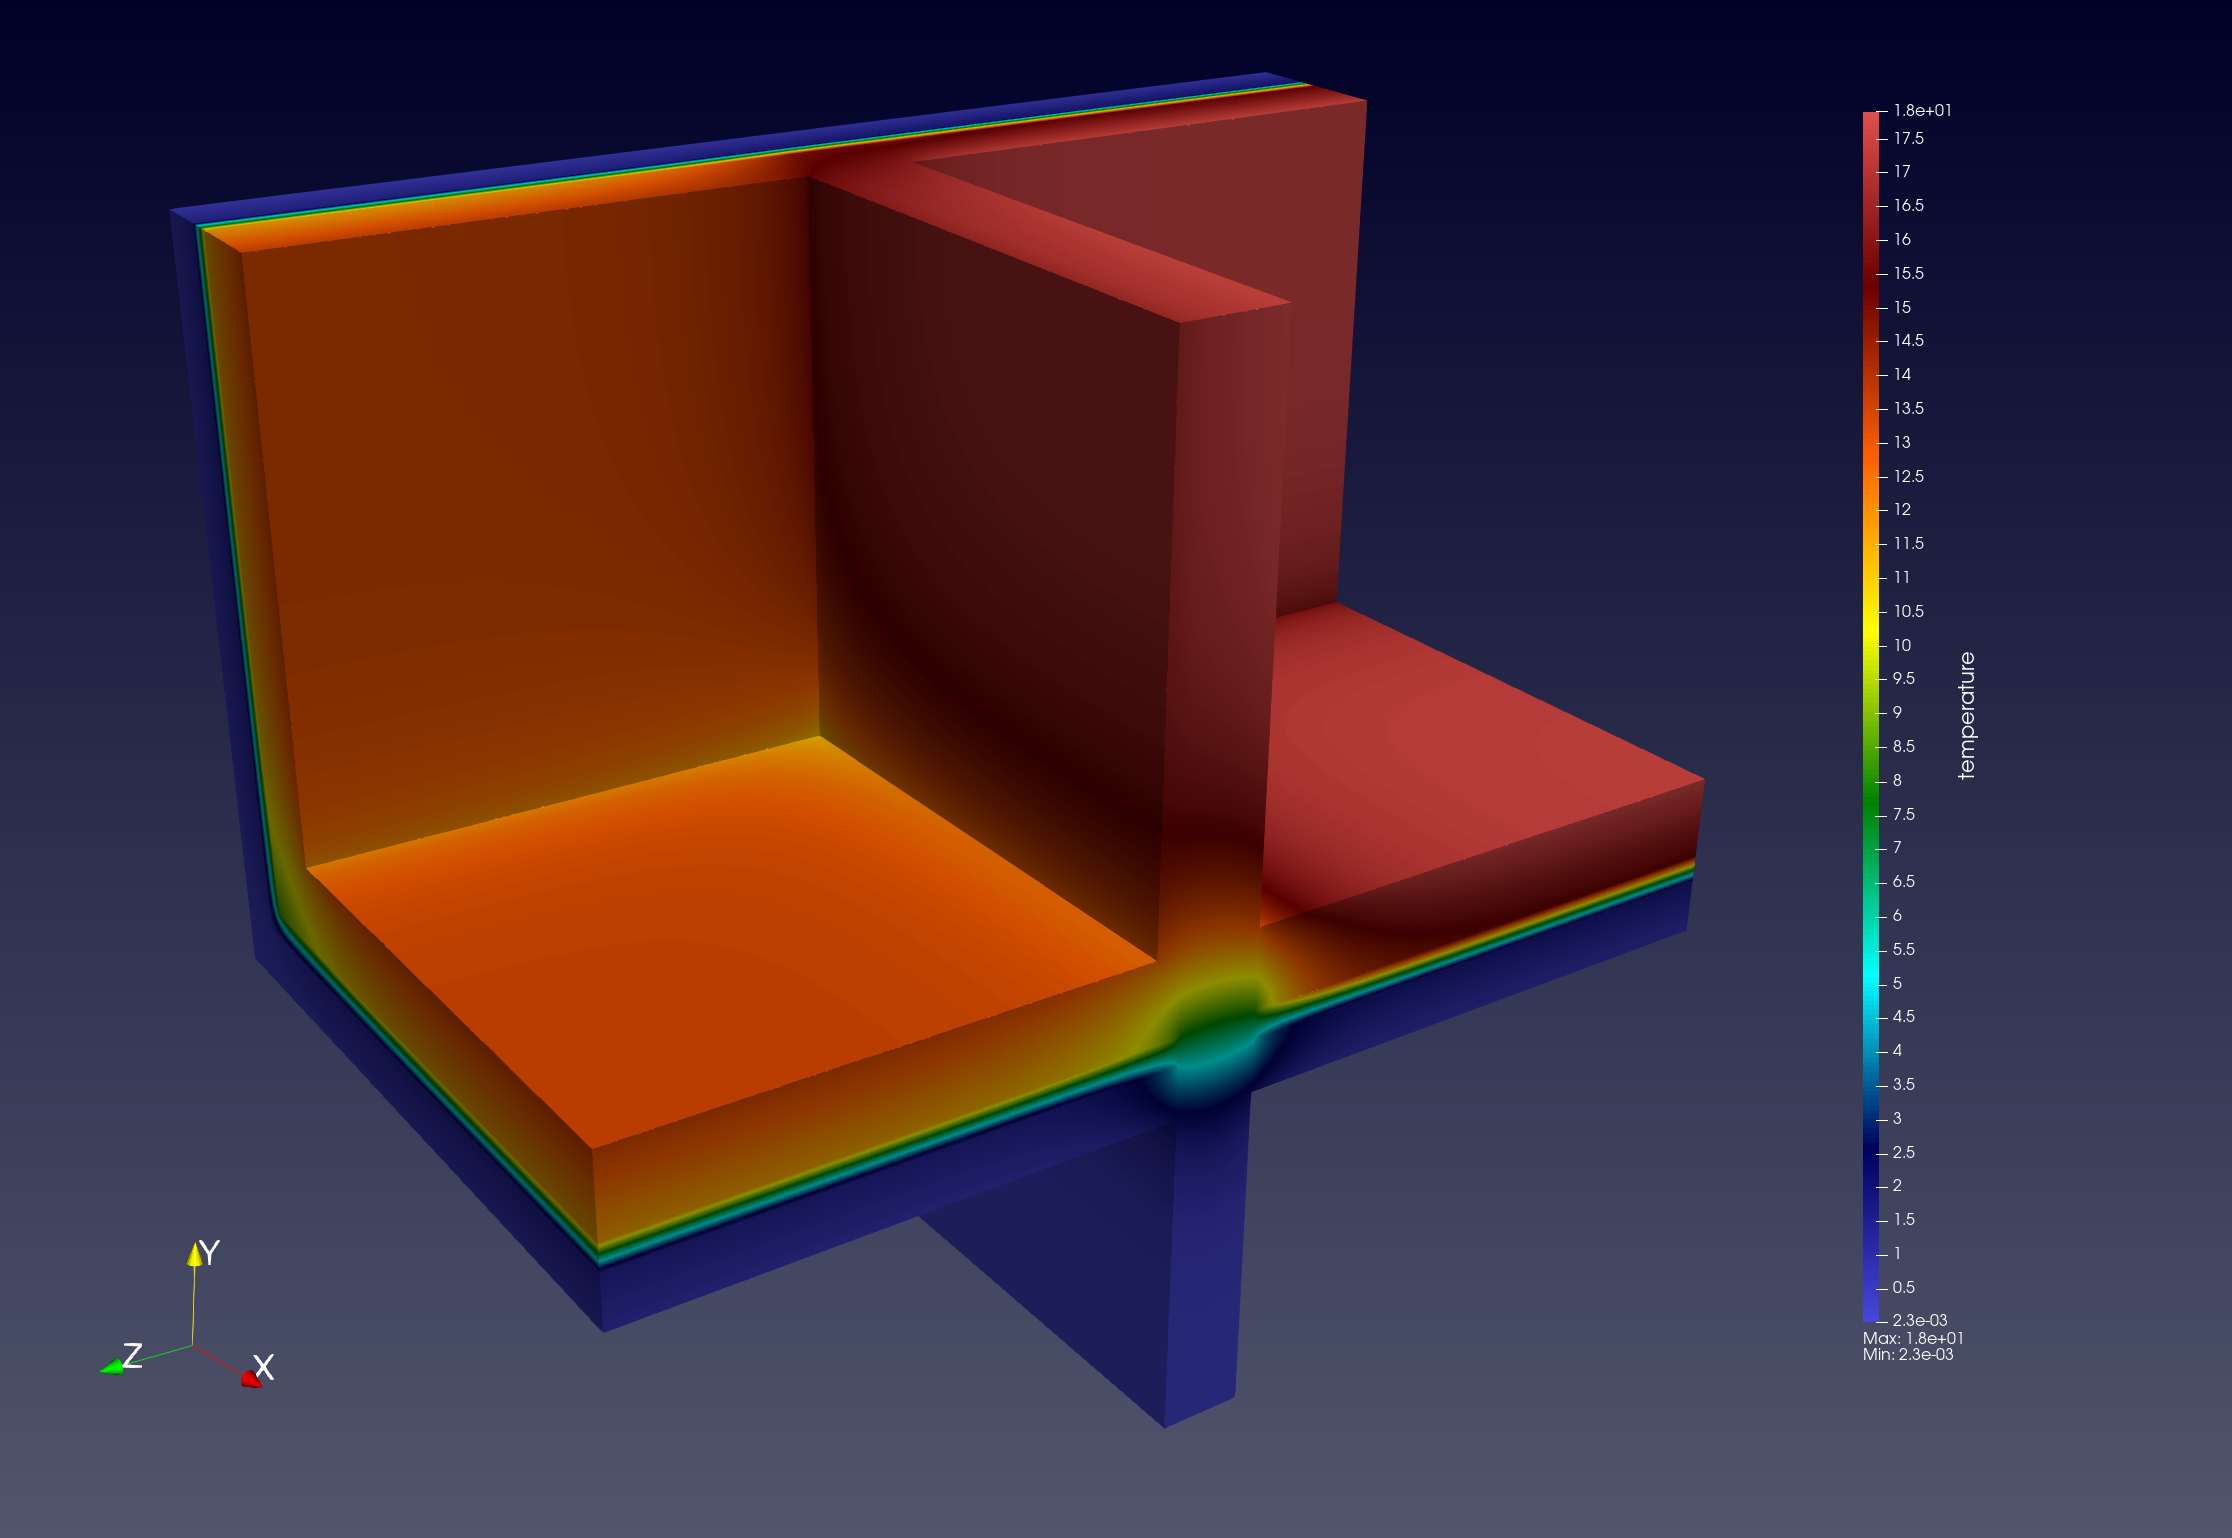
\includegraphics[width=\textwidth]{graphics/feelpp/feelpp-benchmark-thermalbridges-solution.png}
  \end{subfigure}
  \hfill
  \begin{subfigure}[c]{0.49\textwidth}
    \centering
    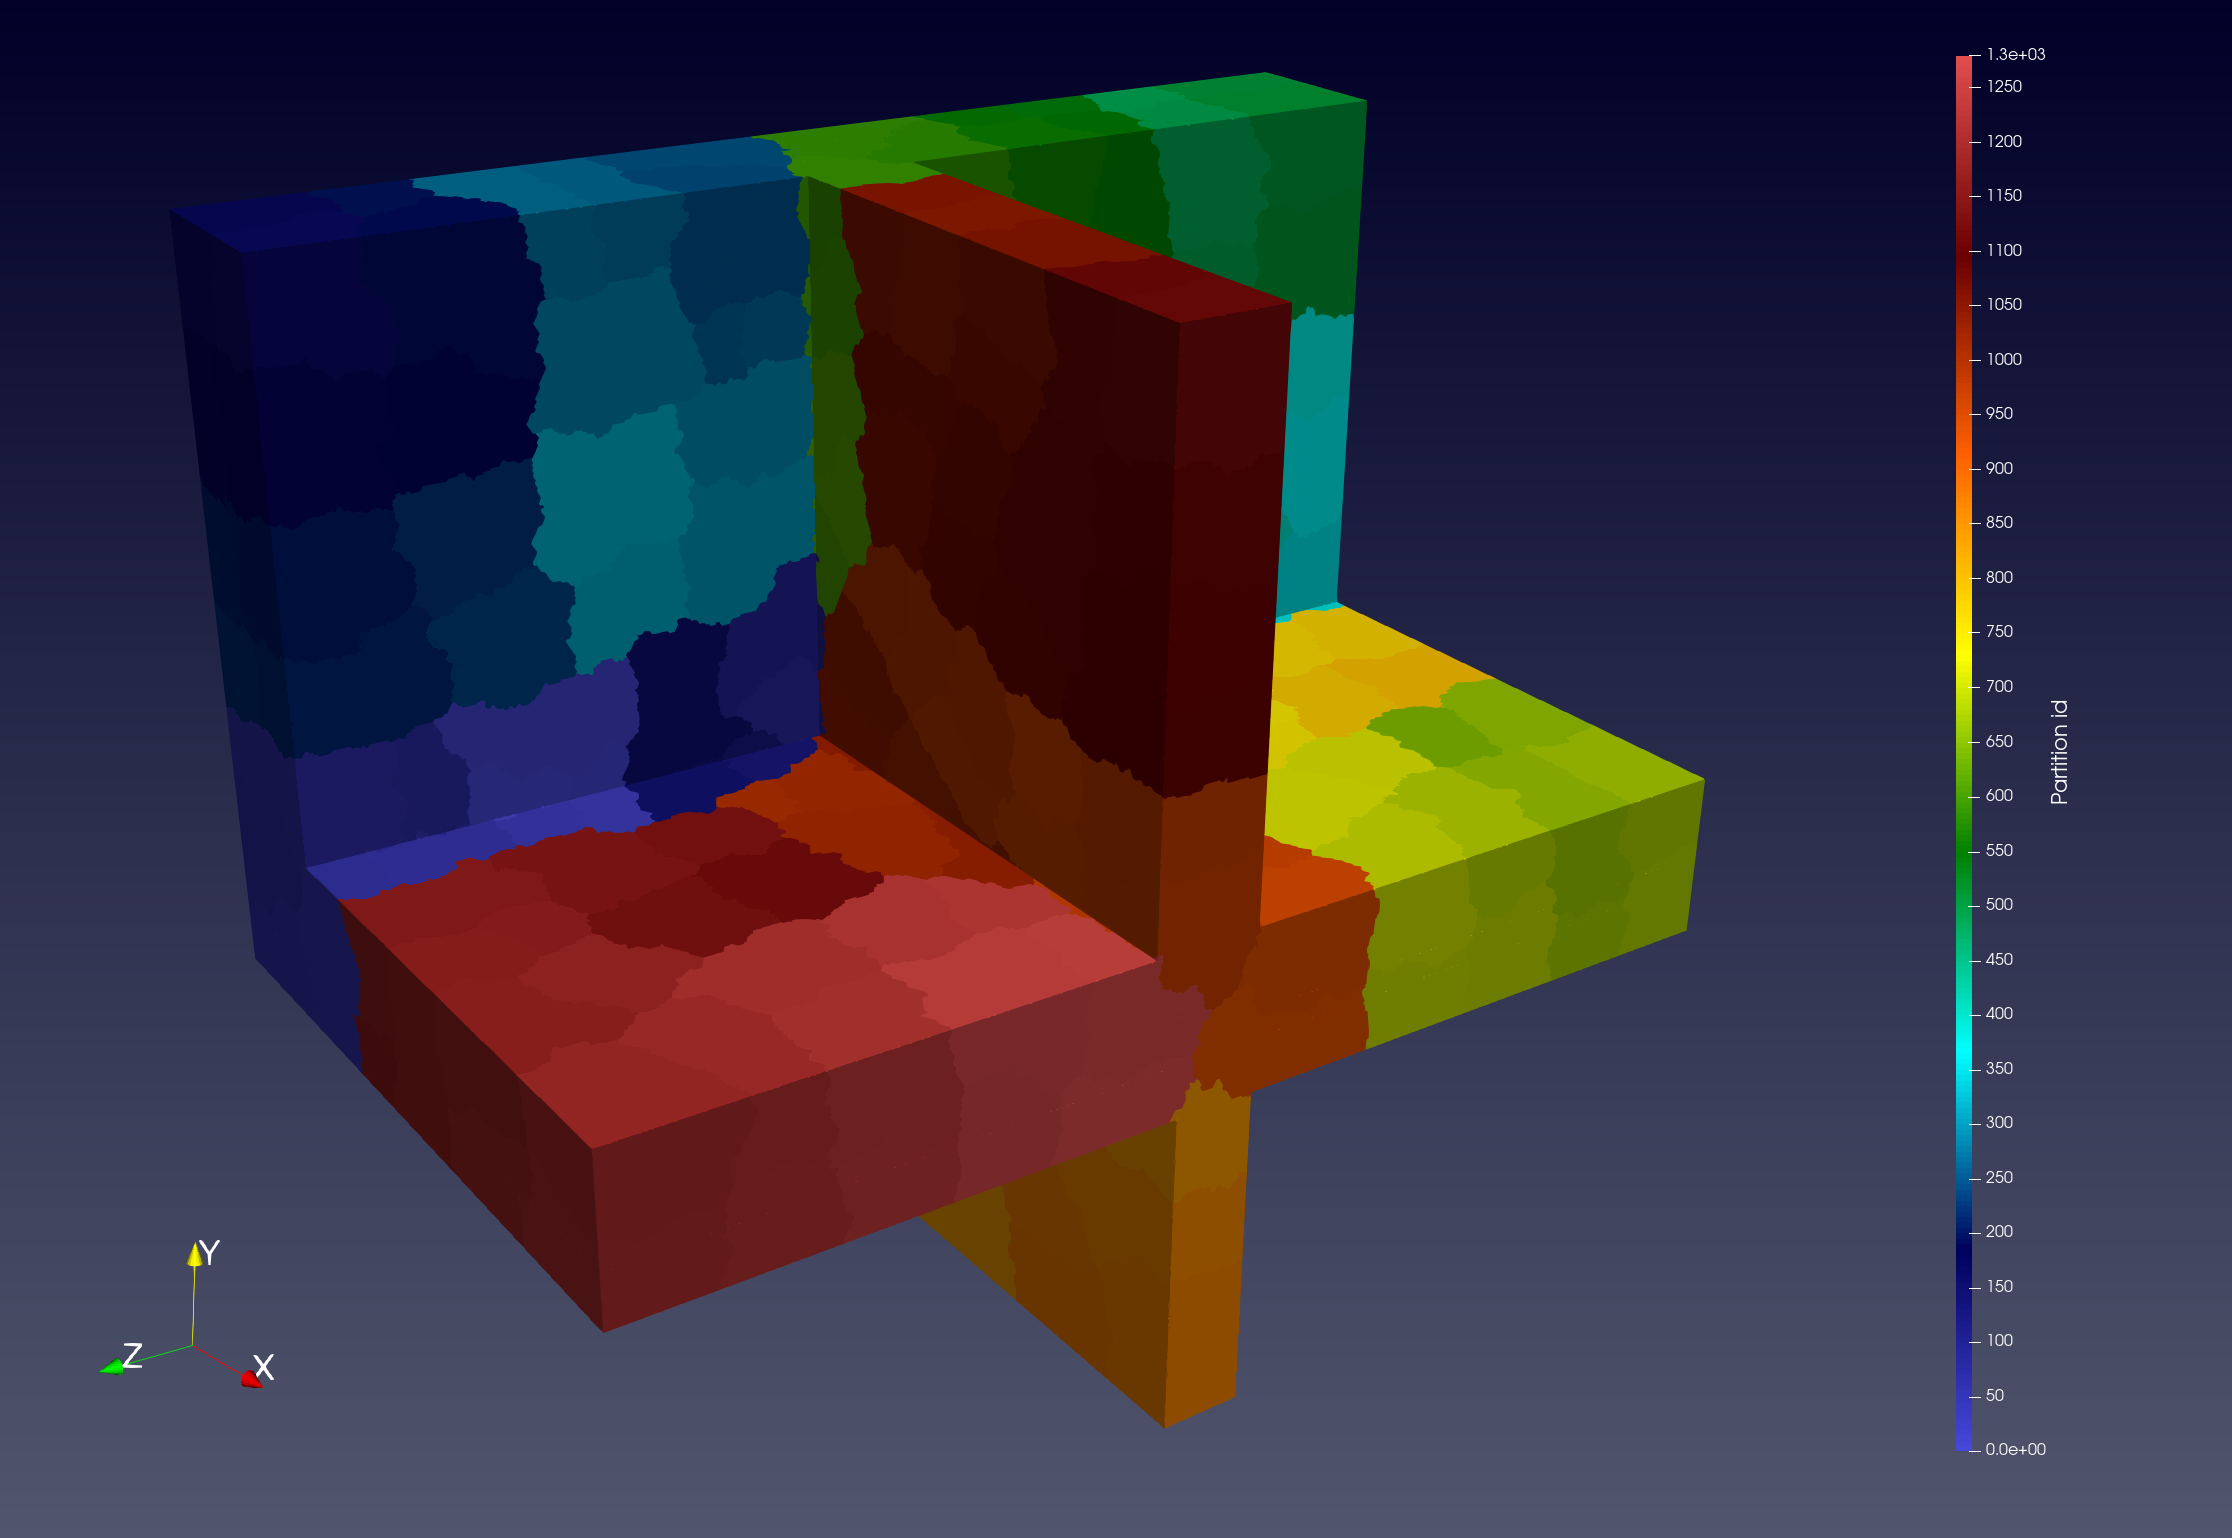
\includegraphics[width=\textwidth]{graphics/feelpp/feelpp-benchmark-thermalbridges-pid.png}
  \end{subfigure}
  \caption{Thermal bridges benchmarks - temperature solution (left) and
    partitioning example (right)}
  \label{fig:wp1:feelpp:thermal_bridges:visualization}
\end{figure}



\paragraph{Benchmarking Tools Used}

The benchmark was performed on the \textbf{Discoverer} supercomputer (see
\Cref{sec:arch:eurohpc-ju}).
The performance tools integrated into the \Feelpp-toolboxes framework were used to measure
the execution time.
Moreover, we need to note that we have used here Apptainer with \Feelpp SIF image based on Ubuntu noble OS.

The metrics measured are the execution time of the main components of the simulation. We enumerate these parts in the following:
\begin{itemize}
\item \textbf{Init}: load mesh from filesystem and initialize heat toolbox (finite element context and algebraic data structure)
\item \textbf{Assembly}: calculate and assemble the matrix and rhs values obtained using the finite element method
\item \textbf{Solve}: the linear system by using a preconditioned gmres
\item \textbf{PostProcess}: compute validation measures (temperature at points and
  heat flux) and export on the filesystem a visualization format (EnsighGold) of
  the solution.
\end{itemize}

\paragraph{Input/Output Dataset Description}

\begin{itemize}
\item \textbf{Input Data:}
  \begin{itemize}
  \item Meshes: We have generated three levels of mesh called M1, M2
    and M3. These meshes are stored in GMSH format. The statistics can be found in
    \Cref{tab:wp1:feelpp:thermal_bridges:discr_stat}. We have also prepared for
    each mesh level a collection of partitioned mesh.
    The format used is an in-house mesh format of \Feelpp based on
    JSON+HDF5 file type.
    The Gmsh meshes and the partitioned meshes can be found on our Girder
    database management, in the \Feelpp collections.
  \item Setup: Use standard setup of \Feelpp toolboxes. It corresponds to a cfg
    file and JSON file. These config files are present in the Github of feelpp.
  \item Sif image: feelpp:v0.111.0-preview.10-noble-sif  (stored in the Github registry of \Feelpp)
  \end{itemize}
\item \textbf{Output Data:} The output includes the computed values of
  validation measure in CSV files format, export visualization files (mesh, partitioning, temperature), and the time taken to perform each simulation step.
\end{itemize}



\begin{table}[h!]
  \centering
  { \setlength{\parindent}{0pt}
    \def\arraystretch{1.25}
    \arrayrulecolor{numpexgray}
    {\fontsize{9}{11}\selectfont
      \begin{tabular}{!{\color{numpexgray}\vrule}c!{\color{numpexgray}\vrule}c!{\color{numpexgray}\vrule}c!{\color{numpexgray}\vrule}c!{\color{numpexgray}\vrule}c!{\color{numpexgray}\vrule}c!{\color{numpexgray}\vrule}c!{\color{numpexgray}\vrule}c!{\color{numpexgray}\vrule}}
        \rowcolor{numpexgray}\multicolumn{5}{c!{\color{numpexgray}\vrule}}{\color{white}\bf Mesh properties}
        & \multicolumn{3}{c!{\color{numpexgray}\vrule}}{\color{white}\bf Number of degrees of freedom} \\
        \rowcolor{numpexgray} {\color{white}\bf Tag} & {\color{white}\bf \# points} & {\color{white}\bf \# edges} & {\color{white}\bf \# faces} & {\color{white}\bf \# elements} & {\color{white}\bf $P_1$} & {\color{white}\bf $P_2$} & {\color{white}\bf $P_3$} \\
        \texttt{M1} & \pgfmathprintnumber{193654} & \pgfmathprintnumber{1299920} & \pgfmathprintnumber{2164759} & \pgfmathprintnumber{1058492} & \pgfmathprintnumber{193654} & \pgfmathprintnumber{1493574} & \pgfmathprintnumber{4958253} \\
        \texttt{M2} & \pgfmathprintnumber{1401135} & \pgfmathprintnumber{9778744} & \pgfmathprintnumber{16566803} & \pgfmathprintnumber{8189193} & \pgfmathprintnumber{1401135} & \pgfmathprintnumber{11179879} & \pgfmathprintnumber{37525426} \\
        \texttt{M3} & \pgfmathprintnumber{10572256} & \pgfmathprintnumber{75307308} & \pgfmathprintnumber{128722252} & \pgfmathprintnumber{63987199} & \pgfmathprintnumber{10572256} & \pgfmathprintnumber{85879564} & \pgfmathprintnumber{289909124} \\
        \hline
      \end{tabular}
    }}
  \caption{Thermal bridges benchmarks - Statistics on meshes and number of degrees of freedom with respect
    to finite element approximation}
  \label{tab:wp1:feelpp:thermal_bridges:discr_stat}
\end{table}


\paragraph{Results Summary}
The benchmark results are summarized in
\Cref{fig:feelpp:wp1:thermal_bridges:performance_times_M1},
\Cref{fig:feelpp:wp1:thermal_bridges:performance_times_M2},
\Cref{fig:feelpp:wp1:thermal_bridges:performance_times_M3} which correspond respectively to
choice of the mesh M1, M2 and M3. Moreover, for each mesh, we have experimented with several
finite element discretizations called $P_1$, $P_2$ and $P_3$.
For each order of finite element approximation, we have selected a set of number
of CPU cores.

Firstly, we can see clearly that the Solve part is the most time-consuming. See
comments in \Cref{sec:WP3:Feelpp:benchmark:thermal_bridges}.
Concerning the mesh M1, considered a coarse mesh, we note that the
scalability scaling is not good, especially for low order. This is simply because the problem is too small for so many HPC resources. MPI
communications an IO effects are non-negligible.
For the mesh M2, results are better (but not ideal) up to around one thousand processing cores.
Finally, the fined mesh M3, illustrates the best scalability on this range of
number of tasks. Except for the solve part, we can see an efficiency of increased
HPC resource at this level.

Each run illustrated here is also validated thanks to the value of the ISO 10211:2017 standard.
With these experiments, we have also seen that we have some variability in
performance measures. Some aspects like the filesystem and network load, are not
under our control, it can explain a part of this. Also, the memory and
consequently the choice of the number of tasks per node can be important and
can change significantly the performance. This latter will be taken into account
more accurately in a next campaign of these benchmarking test.

\newcommand{\barChart}[2][ybar]{
  \begin{tikzpicture}
    \begin{axis}[
      width=\textwidth, height=0.6172\textwidth,
      xlabel={Number of CPU core}, ylabel={Execution time [s]},
      %xticklabels from table={#2}{nProc},
      xtick=data,
      xtick align=outside,
      ymin=0,
      %legend style={at={(1,1)}, anchor=north east},
      %legend style={at={(0.5,1)}, anchor=south,font=\tiny,legend columns=-1},
      ymajorgrids=true, yminorgrids=true,
      bar width=7pt,
      #1
    ]
    \foreach [expand list=true] \thetuple in {#2} {
      \pgfkeys{/mysettings/.cd,
        table/.store in=\mytable,
        column/.store in=\mycolumn,
        shift/.store in=\myshift, shift/.default=0, shift,
        legend/.store in=\mylegend,
        color/.store in=\mycolor
      }
      \edef\temp{
        \noexpand\pgfkeys{/mysettings/.cd, \expandafter\@firstofone\thetuple}
      } \temp
      %\def\toto{\expandafter\mytable}
      \edef\temp{
        \noexpand\addplot[ybar, bar width=0.2, fill=\mycolor, draw=black, point meta=y]
        table [x expr=\noexpand\coordindex+\myshift, y=\mycolumn ] {\expandafter\noexpand\csname \mytable\endcsname};
        %table [x=nProc, y=\mycolumn ] {\expandafter\noexpand\csname \mytable\endcsname};
      } \temp
      %table [x expr=\noexpand\coordindex, y=\mycolumn ] {#2};
      \edef\temp{
        \noexpand\addlegendentry{\mylegend}
      } \temp
    }
    \end{axis}
\end{tikzpicture}
}


\foreach [expand list=true] \meshId in {1,2,3} {

  \pgfplotstableread[col sep=comma]{\currfiledir/data/thermalbridges_M\meshId_P1_discoverer.csv}\dataPa
  \pgfplotstableread[col sep=comma]{\currfiledir/data/thermalbridges_M\meshId_P2_discoverer.csv}\dataPb
  \pgfplotstableread[col sep=comma]{\currfiledir/data/thermalbridges_M\meshId_P3_discoverer.csv}\dataPc

  \begin{figure}
    \centering
    \def\plotSetup##1{
      {table=##1,column=init,legend=Init,color=customdarkblue},
      {table=##1,legend=Assembly,column=algebraic-assembly,color=customcyan},
      {table=##1,legend=Solve,column=algebraic-solve,color=customorange},
      {table=##1,legend=PostProcess,column=exportResults,color=custompurple}
    }
    \def\chartBarPlot##1##2{
      \barChart[ybar,
      xticklabels from table={##2}{nProc},
      legend style={at={(0.5,1)}, anchor=south,font=\tiny,legend columns=-1}
      ]{\plotSetup{##1}}
    }
    \def\chartBarStackedPlot##1##2{
      \barChart[ybar stacked,
      xticklabels from table={##2}{nProc},
      legend style={at={(0.5,1)}, anchor=south,font=\tiny,legend columns=-1}
      ]{\plotSetup{##1}}
    }

    \begin{subfigure}[c]{0.49\textwidth}
      \centering
      \chartBarPlot{dataPa}{\dataPa}
      \caption{\texttt{M\meshId} - \texttt{$P_1$}}
    \end{subfigure}
    \hfill
    \begin{subfigure}[c]{0.49\textwidth}
      \centering
      \chartBarStackedPlot{dataPa}{\dataPa}
      \caption{\texttt{M\meshId} - \texttt{$P_1$}}
    \end{subfigure}
    \hfill
    \begin{subfigure}[c]{0.49\textwidth}
      \centering
      \chartBarPlot{dataPb}{\dataPb}
      \caption{\texttt{M\meshId} - \texttt{$P_2$}}
    \end{subfigure}
    \hfill
    \begin{subfigure}[c]{0.49\textwidth}
      \centering
      \chartBarStackedPlot{dataPb}{\dataPb}
      \caption{\texttt{M\meshId} - \texttt{$P_2$}}
    \end{subfigure}
    \hfill
    \begin{subfigure}[c]{0.49\textwidth}
      \centering
      \chartBarPlot{dataPc}{\dataPc}
      \caption{\texttt{M\meshId} - \texttt{$P_3$}}
    \end{subfigure}
    \hfill
    \begin{subfigure}[c]{0.49\textwidth}
      \centering
      \chartBarStackedPlot{dataPc}{\dataPc}
      \caption{\texttt{M\meshId} - \texttt{$P_3$}}
    \end{subfigure}
    \caption{Thermal bridges benchmarks - Execution time of main simulation components
      - Mesh \texttt{M\meshId} - Discoverer supercomputer}
    \label{fig:feelpp:wp1:thermal_bridges:performance_times_M\meshId}
  \end{figure}

}




% columns/FunctionSpace/.style={string type},
\begin{figure}
  \centering
  \captionsetup[subfigure]{justification=centering}

  \pgfplotstableread[col sep=comma]{\currfiledir/data/measures_all.csv}\dataTableMeasures
  \def\myLineWidth{2pt}
  \def\myLineStyleA{loosely dashdotdotted} %dashdotdotted
  \def\myLineStyleB{dashed}
  \def\myLineStyleC{solid}

  \def\myAddPlot#1#2#3#4{
    \addplot[#3,every mark/.append style={solid},
    % x filter/.expression={(\thisrow{PolyOrder} == 1 ?  \pgfmathparse{\thisrow{Mesh}}\pgfmathresult :NaN)},
    % x filter/.expression={ \thisrow{FunctionSpace} == \thisrow{FunctionSpace} ? \pgfmathresult
    % x filter/.expression={(\thisrow{FunctionSpace} == P1 ? \pgfmathresult :NaN )},
    x filter/.code={
      \pgfmathparse{\thisrow{PolyOrder}==#2}
      \ifnum0=\pgfmathresult
      \pgfmathsetmacro{\newx}{nan}
    \else
      \pgfmathsetmacro{\newx}{\thisrow{Mesh}}
    \fi
    \pgfmathparse{\newx}
  },
  y filter/.expression={ #4*\pgfmathresult }
  ] table [x=Mesh, y=#1] {\dataTableMeasures};
  }

  \def\myPlotOutputMeasures#1#2#3#4{
      \resizebox{\textwidth}{0.6172\textwidth}{
    \begin{tikzpicture}
    \begin{axis}[
      %width=\textwidth, height=1.2\textheight,
      xtick=data,
      xticklabel={M$\pgfmathprintnumber{\tick}$},
      xmajorgrids=true,% xminorgrids=false, minor x tick num=3,
      ymajorgrids=true, yminorgrids=true,
      minor y tick num=2,
      % xticklabel={\pgfmathparse{100*\tick}\pgfmathprintnumber[precision=0]{\pgfmathresult}\%},
      %xticklabel={\pgfmathparse{\tick}\pgfmathprintnumber[fixed,set thousands separator={},precision=0]{\pgfmathresult}},
      xlabel={Mesh levels}, ylabel={#4},
      % legend style={at={(0.5,1)}, anchor=south,font=\small,legend columns=3}
      %legend style={at={(0.,1)}, anchor=north west,font=\small,legend
      %columns=3},
      legend style={at={(0.,1)}, anchor=south west,font=\small,legend columns=4},
      %#2
      ]

      \myAddPlot{#1}{1}{color=customdarkblue,\myLineStyleC,mark=o,line width=\myLineWidth}{#2}
      \addlegendentry{P1}
      \myAddPlot{#1}{2}{color=customcyan,\myLineStyleC,mark=triangle,line width=\myLineWidth}{#2}
      \addlegendentry{P2}
      \myAddPlot{#1}{3}{color=customorange,\myLineStyleC,mark=square,line width=\myLineWidth}{#2}
      \addlegendentry{P3}
      \addplot+[color=red,\myLineStyleB,mark=none,line width=\myLineWidth,every mark/.append style={solid}] coordinates {
        (1,#3) (3,#3)
      };
      \addlegendentry{Ref}

    \end{axis}
  \end{tikzpicture}
      }

}

  \begin{subfigure}[c]{0.49\textwidth}
    \centering
    \myPlotOutputMeasures{Normal_Heat_Flux_alpha}{1}{46.09}{Heat flow [W]}
    \caption{Heat flow measured in $\alpha$ environment}
  \end{subfigure}
  \hfill
  \begin{subfigure}[c]{0.49\textwidth}
    \centering
    \myPlotOutputMeasures{Normal_Heat_Flux_beta}{1}{13.89}{Heat flow [W]}
    \caption{Heat flow measured in $\beta$ environment}
  \end{subfigure}
  \hfill
  \begin{subfigure}[c]{0.49\textwidth}
    \centering
    \vspace*{0.03\textheight}
    \myPlotOutputMeasures{Normal_Heat_Flux_gamma}{-1}{59.98}{Heat flow [W]} % warning inverse
    \caption{Heat flow measured in $\gamma$ environment}
  \end{subfigure}
  \hfill
  \begin{subfigure}[c]{0.49\textwidth}
    \centering
    \vspace*{0.03\textheight}
    \myPlotOutputMeasures{Statistics_temperature_alpha_min}{1}{11.32}{Temperature
      [°C]}
    \caption{Surface temperature min in $\alpha$ environment}
  \end{subfigure}

  \caption{Thermal bridges benchmarks - Convergence of validation measures compared to references values}
    \label{fig:feelpp:wp1:thermal_bridges:measures_convergences}
\end{figure}



\paragraph{Challenges Identified}
Several challenges were encountered during the benchmarking process:
\begin{itemize}
    \item \textbf{Memory Usage:} We need to check and detect the memory
      consumed during the simulation to avoid bad behavior like swapping.
    \item \textbf{Parallelization Inefficiencies:} We need to understand and
      improve performance when MPI communication and filesystem IO will be dominant.
    %\item \textbf{Cache and Memory Bottlenecks:}
\end{itemize}

To conclude, we have realized HPC performance tests of benchmark called thermal
bridges. We have realized with success the execution of several simulations on
significant resources and demonstrated the validation of \Feelpp framework in the
elliptic PDE context. We have also validated the deployment of \Feelpp with
container support. Now, we need to provide more refined measures to detect and
analyze reasons for performance degradation. And also compare to other software
installations, like Spack.



\subsubsection{Benchmark \#2: Linear elasticity : NAFEMS LE10}

\paragraph{Description}

\begin{figure}[h]
  \centering
  \begin{subfigure}[c]{0.49\textwidth}
    \centering
    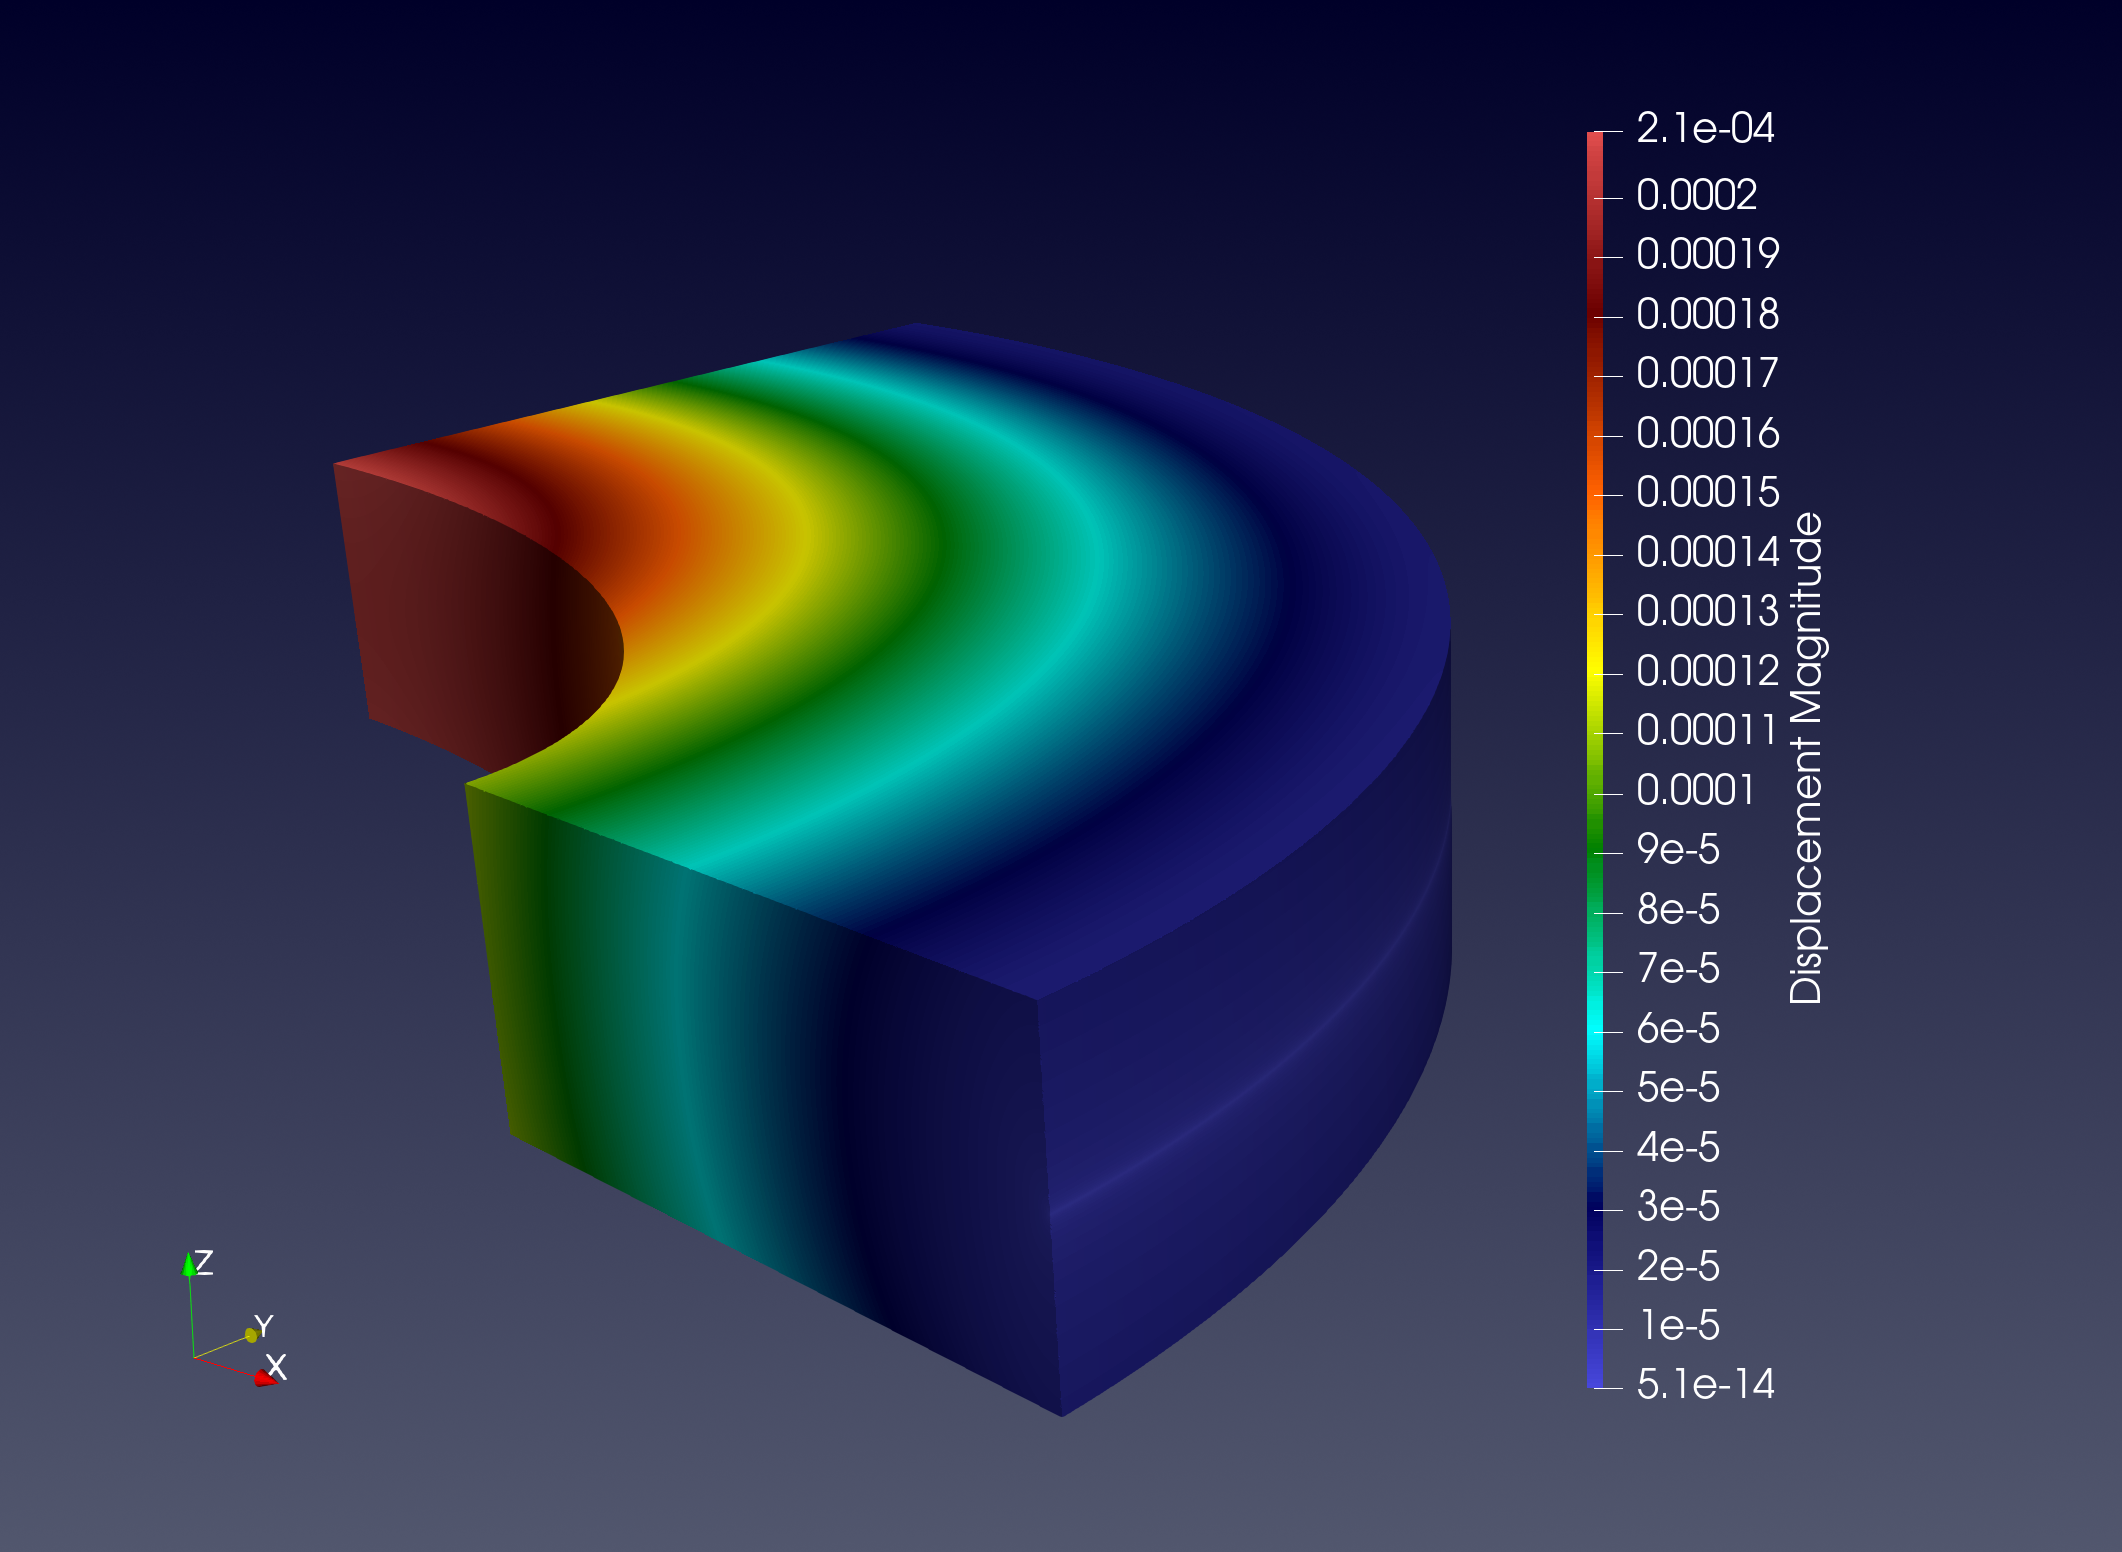
\includegraphics[width=\textwidth]{graphics/feelpp/feelpp-benchmark-nafems-le10-solution-disp.png}
  \end{subfigure}
  \hfill
  \begin{subfigure}[c]{0.49\textwidth}
    \centering
    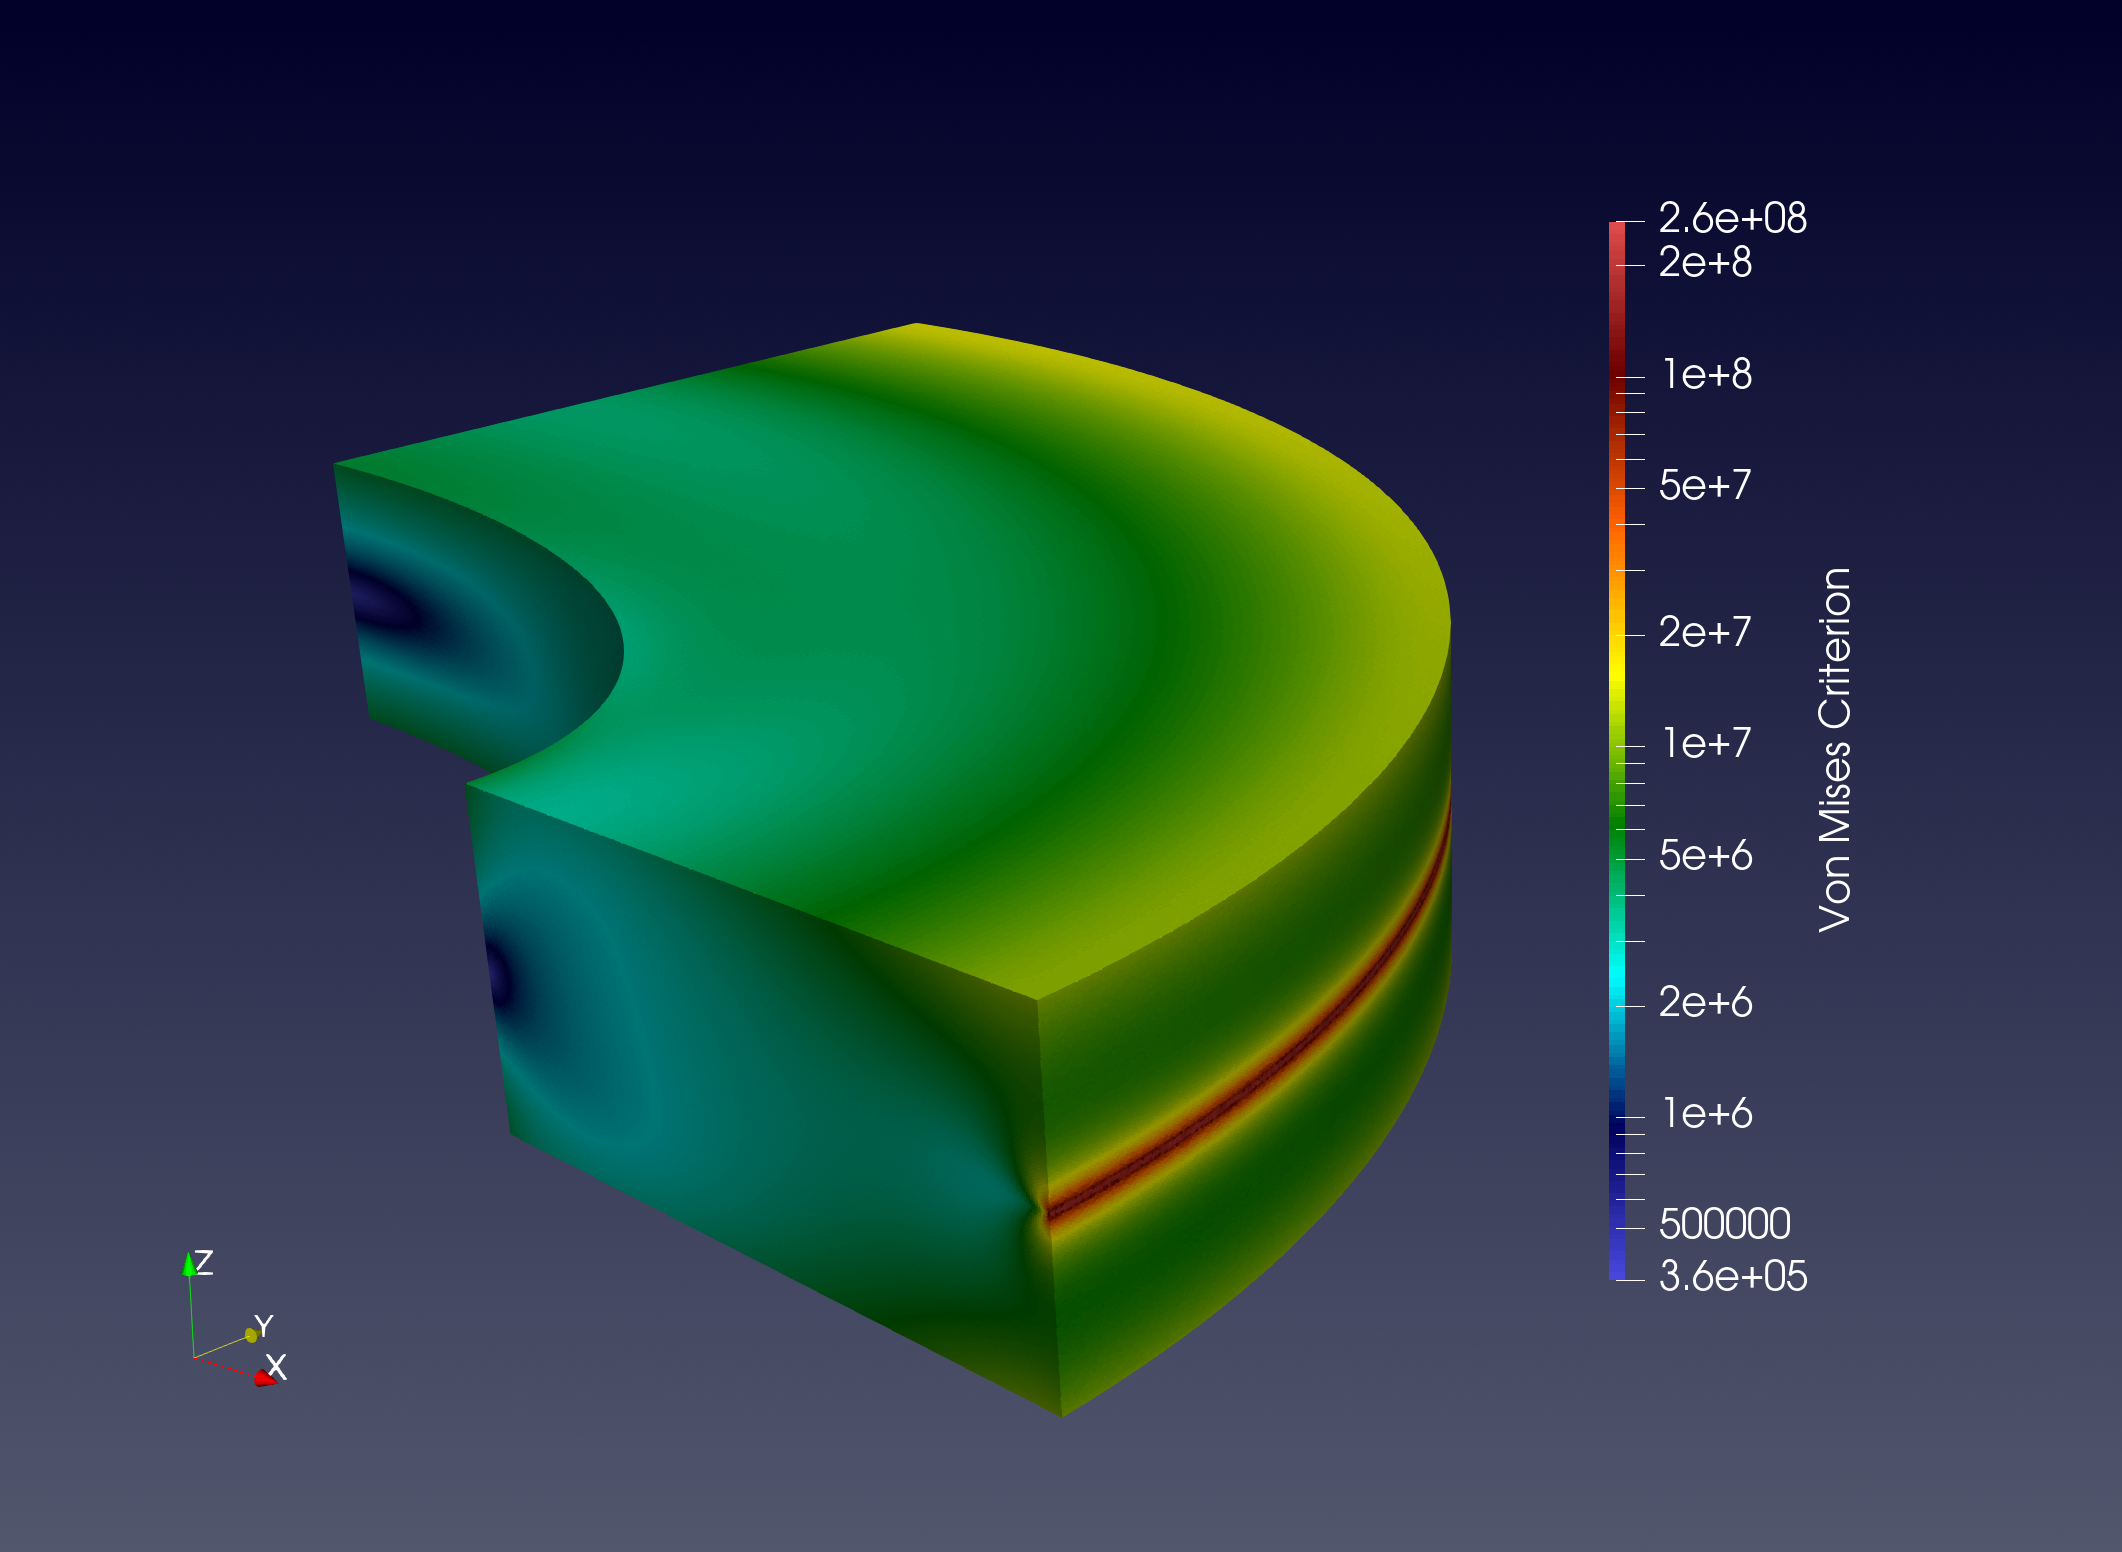
\includegraphics[width=\textwidth]{graphics/feelpp/feelpp-benchmark-nafems-le10-solution-vonmises.png}
  \end{subfigure}
  \caption{Thermal bridges benchmarks - displace solution (left) and
    von Mises yield criterion (right)}
  \label{fig:wp1:feelpp:nafems-le10:visualization}
\end{figure}

\paragraph{Benchmarking Tools Used}

\paragraph{Input/Output Dataset Description}

\begin{table}[h!]
  \centering
  { \setlength{\parindent}{0pt}
    \def\arraystretch{1.25}
    \arrayrulecolor{numpexgray}
    {\fontsize{9}{11}\selectfont
      \begin{tabular}{!{\color{numpexgray}\vrule}c!{\color{numpexgray}\vrule}c!{\color{numpexgray}\vrule}c!{\color{numpexgray}\vrule}c!{\color{numpexgray}\vrule}c!{\color{numpexgray}\vrule}c!{\color{numpexgray}\vrule}c!{\color{numpexgray}\vrule}c!{\color{numpexgray}\vrule}}
        \rowcolor{numpexgray}\multicolumn{5}{c!{\color{numpexgray}\vrule}}{\color{white}\bf Mesh properties}
        & \multicolumn{2}{c!{\color{numpexgray}\vrule}}{\color{white}\bf Number of degrees of freedom} \\
        \rowcolor{numpexgray} {\color{white}\bf Tag} & {\color{white}\bf \# points} & {\color{white}\bf \# edges} & {\color{white}\bf \# faces} & {\color{white}\bf \# elements} & {\color{white}\bf $P_1$} & {\color{white}\bf $P_2$} \\
        \texttt{M2} & \pgfmathprintnumber{324257} & \pgfmathprintnumber{2247489} & \pgfmathprintnumber{3796235} & \pgfmathprintnumber{1873002} & \pgfmathprintnumber{972771} & \pgfmathprintnumber{7715238}  \\
        \texttt{M3} & \pgfmathprintnumber{2426377} & \pgfmathprintnumber{17230019} & \pgfmathprintnumber{29409215} & \pgfmathprintnumber{14605572} & \pgfmathprintnumber{7279131} & \pgfmathprintnumber{58969188}  \\
        \texttt{M4} & \pgfmathprintnumber{18801264} & \pgfmathprintnumber{135213828} & \pgfmathprintnumber{232036941} & \pgfmathprintnumber{115624376} & \pgfmathprintnumber{56403792} & \pgfmathprintnumber{462045276} \\
        \hline
      \end{tabular}
    }}
  \caption{NAFEMS le10 benchmark - Statistics on meshes and number of degrees of freedom with respect
    to finite element approximation}
  \label{tab:wp1:feelpp:nafems-le10:discr_stat}
\end{table}

\paragraph{Results Summary}

\foreach [expand list=true] \meshId in {2,3,4} {

  \pgfplotstableread[col sep=comma]{\currfiledir/data/nafems_le10_M\meshId_P1_discoverer.csv}\dataPa
  \pgfplotstableread[col sep=comma]{\currfiledir/data/nafems_le10_M\meshId_P2_discoverer.csv}\dataPb

  \begin{figure}
    \centering
    \def\plotSetup##1{
      {table=##1,column=init,legend=Init,color=customdarkblue},
      {table=##1,legend=Assembly,column=algebraic-assembly,color=customcyan},
      %{table=##1,legend=Solve,column=algebraic-solve,color=customorange},
      {table=##1,legend=PostProcess,column=exportResults,color=custompurple}
    }
    \def\chartBarPlot##1##2##3{
      \barChart[ybar,xticklabels from table={##2}{nProc},legend style={at={(0.5,1)}, anchor=south,font=\tiny,legend columns=-1},##3]{\plotSetup{##1}}
    }
    \def\chartBarStackedPlot##1##2{
      \barChart[ybar stacked,xticklabels from table={##2}{nProc},
      legend style={at={(0.5,1)}, anchor=south,font=\tiny,legend columns=-1}
      ]{\plotSetup{##1}}
    }

    \begin{subfigure}[c]{0.49\textwidth}
      \centering
      \chartBarPlot{dataPa}{\dataPa}{}
      \caption{\texttt{M\meshId} - \texttt{$P_1$}}
    \end{subfigure}
    \hfill
    \begin{subfigure}[c]{0.49\textwidth}
      \centering
      \chartBarStackedPlot{dataPa}{\dataPa}
      \caption{\texttt{M\meshId} - \texttt{$P_1$}}
    \end{subfigure}
    \hfill
    \begin{subfigure}[c]{0.49\textwidth}
      \centering
      \ifnum4=\meshId
      \chartBarPlot{dataPb}{\dataPb}{enlarge x limits=0.3}
    \else
      \chartBarPlot{dataPb}{\dataPb}{}
    \fi



      \caption{\texttt{M\meshId} - \texttt{$P_2$}}
    \end{subfigure}
    \hfill
    \begin{subfigure}[c]{0.49\textwidth}
      \centering
      \chartBarStackedPlot{dataPb}{\dataPb}
      \caption{\texttt{M\meshId} - \texttt{$P_2$}}
    \end{subfigure}
    \caption{NAFEMS le10 benchmarks - Execution time of main simulation components
      - Mesh \texttt{M\meshId} - Discoverer supercomputer}
    \label{fig:feelpp:wp1:nafems-le10:performance_times_M\meshId}
  \end{figure}

}
